\subsection{Künstliche neuronale Netzwerke}
\label{sec:KNN}
Künstliche neuronale Netze sind ein Forschungsgebiet der \textit{künstlichen Intelligenz} und imitieren die Beschaffenheit natürlicher neuronale Netze, um komplexe Probleme zu lösen. Inspiriert von ihren biologischen Vorbildern\footnote{das Nervensystem eines komplexen Lebewesens; z.B. des Menschen}, vernetzen künstliche neuronale Netzwerke (\textit{KNN}) künstliche Neuronen miteinander \cite{CS231nConvolutionalNeural}. Dabei kann die Verbindung unidirektional (\textit{feedforward}) oder bidirektional (\textit{feedback}) sein  \cite{Goodfellow-et-al-2016}. 

Bei einem feedforward Netzwerk werden die Daten im Netz immer vorwärts übertragen, hingegen kann ein feedback Netzwerk, auch bekannt als \textit{Recurrent Neural Networks}, Daten rückwärts, sowie in einer Schleife zum selben Neuron, übergeben \cite{Goodfellow-et-al-2016}. Da feedback Netzwerke keinen Einsatz in dieser Arbeit haben, ist im weiteren Verlauf dieser Arbeit bei einem Netzwerk immer ein feedforward Ansatz gemeint. In diesem Kapitel werden als Nächstes ein künstliches Neuron definiert und anschließend ein feedforward Netzwerk beschrieben. Convolutional Neural Networks sind eine besondere Art von künstlichen neuronalen Netzen und bilden einen sehr wichtigen Bestand dieser Arbeit. Daher werden CNNs ein eigener Abschnitt gewidmet, siehe Abschnitt \ref{sec:CNN} .


\subsubsection{Künstliches Neuron}
Ein einzelnes Neuron erhält einen Inputsignal auf mehreren Kanälen und löst erst ein Signal (\textit{output}) aus, falls die gewichtete Summe des Inputs einen gewissen Schwellwert erreicht \cite{CS231nConvolutionalNeural}. Abbildung \ref{fig:neuron} stellt eine beispielhafte Visualisierung eines künstlichen Neurons dar.

Ein künstliches Neuron mit der Inputgröße $M$ ist mathematisch die nicht-lineare Funktion $y : \mathbb{R}^M \mapsto \mathbb{R}$ mit den Parametern $x$ als Input, $w$ als Gewichtsvektor, $b$ als ein Bias, $\phi$ als eine nicht-lineare \textit{Aktivierungsfunktion} \cite{CS231nConvolutionalNeural}:
\begin{equation}
	\label{eq:neuron}
	y(x)=\phi\left(\sum_{m=1}^{M} w_{i} x_{i} + b\right) = \phi(W^Tx+b)
\end{equation}

\vspace*{0.5cm}

\begin{figure}[H]
	\centering
	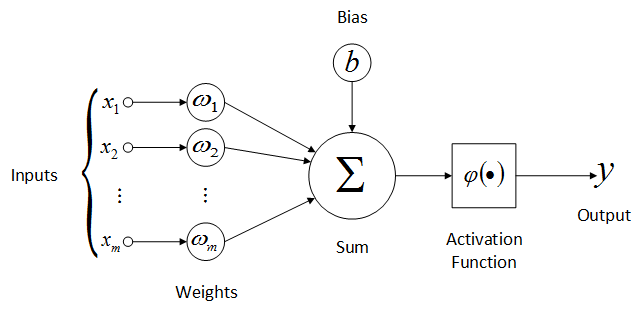
\includegraphics[width=0.8\textwidth]{images/ann_conv/neuron.png}
	\caption{Visualisierung eines künstlichen Neurons definiert nach der Gleichung \ref{eq:neuron}. Dieser Neuron summiert das Produkt des Inputvektors $x$  mit den jeweiligen Gewichten $w$ und addiert einen Bias $b$. Durch die Summe erzeugt die Aktivierungsfunktion $\phi$ das Output $y$ des Neurons. Abbildung \ref{fig:relu} zeigt ein Beispiel für eine Aktivierungsfunktion. Entnommen aus \cite{deoliveiraSystemBasedArtificial2017}. }
	\label{fig:neuron}
\end{figure}

\subsubsection{Feedforward Neural Networks}
\label{sec:feedforwardNN}
Künstliche Neuronen können zu einem Schicht (\textit{layer}) zusammengeführt werden. Die Verbindung solcher Schichten bildet ein neuronales Netzwerk.
Bei einem feedforward (\textit{fully-connected}) Netzwerk übergibt jedes Neuron aus der Schicht $l$ seinen Output $y_{l}$ an jedem Neuron der Schicht $l+1$ weiter. Ebenso sind Neuronen aus der gleichen Schicht untereinander nicht verbunden \cite{Goodfellow-et-al-2016}.
Die Schicht $l$ eines feedforward Netzwerkes operiert somit auf das Ouput $y_{l-1}$ und stellt die nicht-lineare Funktion $f_l :  \mathbb{R}^{M_{l-1}} \mapsto \mathbb{R}^{M_l}$ dar \cite{bauckhageInformedMachineLearning}:
\begin{equation}
\label{eq:layer}
y_l = f_l(y_{l-1}) = \phi(W^T_lx_{l-1}+b_{l})
\end{equation}


Die erste Schicht eines Netzwerks wird als Input-, die letzte Schicht als Ouput Layer bezeichnet. Alle Schichten dazwischen sind Hidden Layer \cite{Goodfellow-et-al-2016}. Der Ouput Layer liefert zugleich auch das Ergebnis eines Netzwerks, daher haben die Neuronen des Ouput Layers grundsätzlich keine Aktivierungsfunktion \cite{CS231nConvolutionalNeural}.

Die Tiefe (\textit{depth}) eines Netzwerks ist gegeben durch die Anzahl der Layer \footnote{der Input Layer ist ausgeschlossen} und die Breite (\textit{width}) eines Layers wird durch die Anzahl der Neuronen bestimmt \cite{Goodfellow-et-al-2016}. 
Abbildung \ref{fig:neural_net} illustriert ein feedforward neuronales Netz als ein azyklischer Graph.

Ziel eines KNNs ist es eine Funktion $f^*$ zu approximieren, dass einen Input $x$ auf einen Output $y$ abbildet. Durch das Output $y$ kann das Input $x$ klassifiziert oder anhand dessen ein Wert regressiert werden. Sei $y = f(x; \theta)$ eine derartige Funktion, dann besetzt ein KNN die Werte des $\theta$ Parameters mit eines der besten Approximierung von $f^*$. Der Parameter $\theta$ stellt hierbei die Gewichte dar, die erlernt werden sollen \cite{Goodfellow-et-al-2016}. 
Das Lernen ist die strategische Anpassung der Gewichte über Input-Output Paare (\textit{Trainingsdaten}) und findet grundsätzlich durch ein \textit{Backpropagation}-Verfahren statt \cite{Goodfellow-et-al-2016}. 

Die Funktion $y = f(x; \theta)$ bildet sich aus den Funktionen der im Netzwerk vorhandenen Schichten (Gleichung \ref{eq:layer}) und kann bei einer Tiefe $L$ repräsentiert werden als die folgende Funktion $f :  \mathbb{R}^{M_0} \mapsto \mathbb{R}^{M_L}$ \cite{Goodfellow-et-al-2016, bauckhageInformedMachineLearning}:
 
\begin{equation}
\label{eq:network}
y = f(x; \theta)=  f_L(...f_2(f_1(x))) = (f_L * ... * f_2 * f_1)(x)
\end{equation}

\vspace*{1.5cm}

\begin{figure}[H]
	\centering
	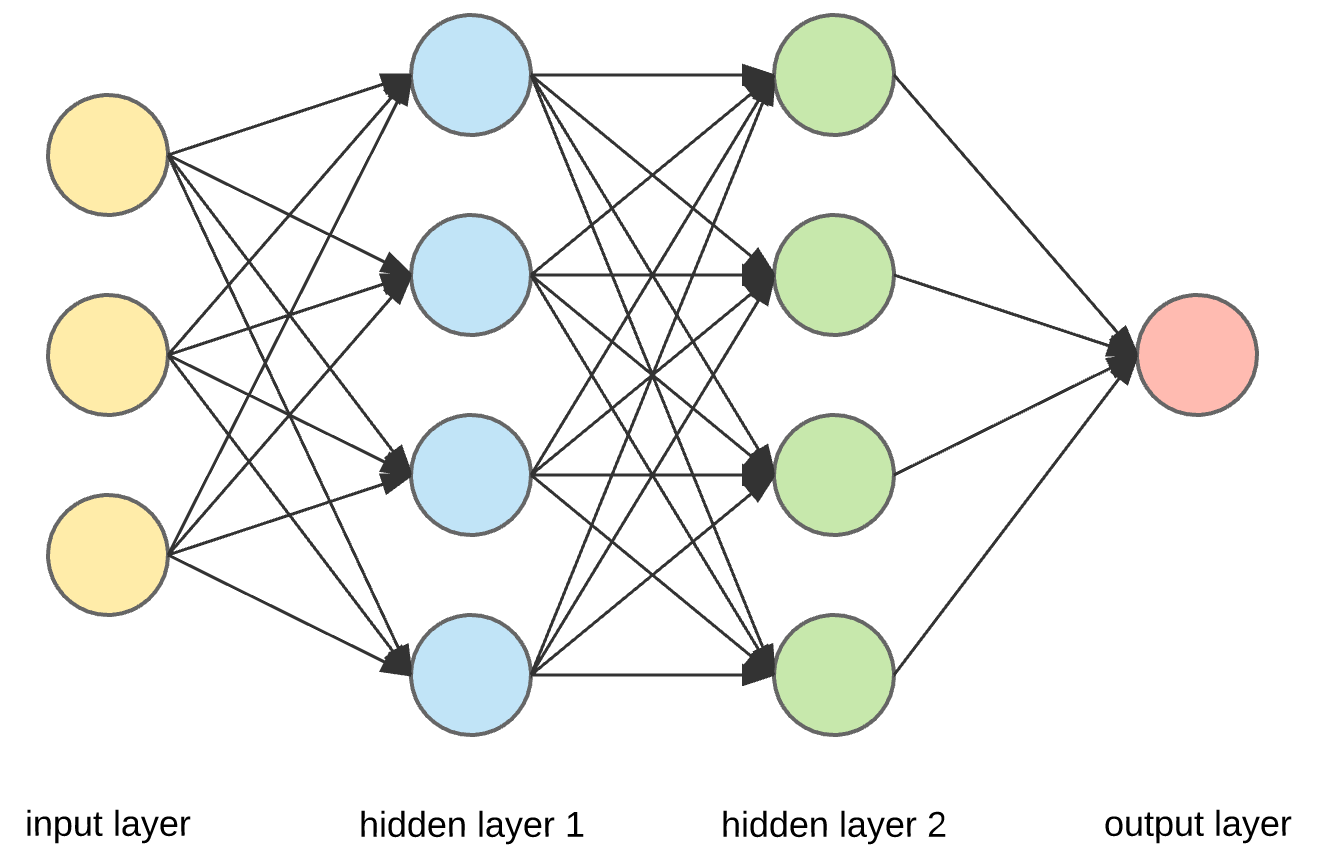
\includegraphics[width=0.6\textwidth]{images/ann_conv/neural_net.png}
	\caption{Ein feedforward neuronales Netz mit der Tiefe 3, bestehend aus einem Input Layer der Breite 3, aus zwei Hidden Layer der Breite 4 und einem Output Layer der Breite 1. Mit der Gleichung \ref{eq:network}  lässt sich dieses Netzwerk als die Funktion $f :  \mathbb{R}^{3} \mapsto \mathbb{R}^{1}$ mit $f(x)=f_3(f_2(f_1(x)))$ darstellen. }
	\label{fig:neural_net}
\end{figure}

\subsection{Convolutional Neural Networks}
\label{sec:CNN}
Einfache neuronale Netze, wie sie in Abschnitt \ref{sec:KNN} beschrieben werden, arbeitet auf einem Inputvektor $x \in \mathbb{R}^{M}$. Im Vergleich dazu arbeiten CNNs auf einem drei-dimensionalen Inputvolumen $x \in \mathbb{R}^{width} \times \mathbb{R}^{heigth} \times \mathbb{R}^{depth}$. CNNs werden hauptsächlich im Kontext von Bildern eingesetzt, dabei stellt z.B. ein 32 $\times$ 32 RGB-Bild ein Volumen von 32 $\times$ 32 $\times$ 3 dar \cite{CS231nConvolutionalNeurala}.

\begin{figure}[H]
	\centering
%	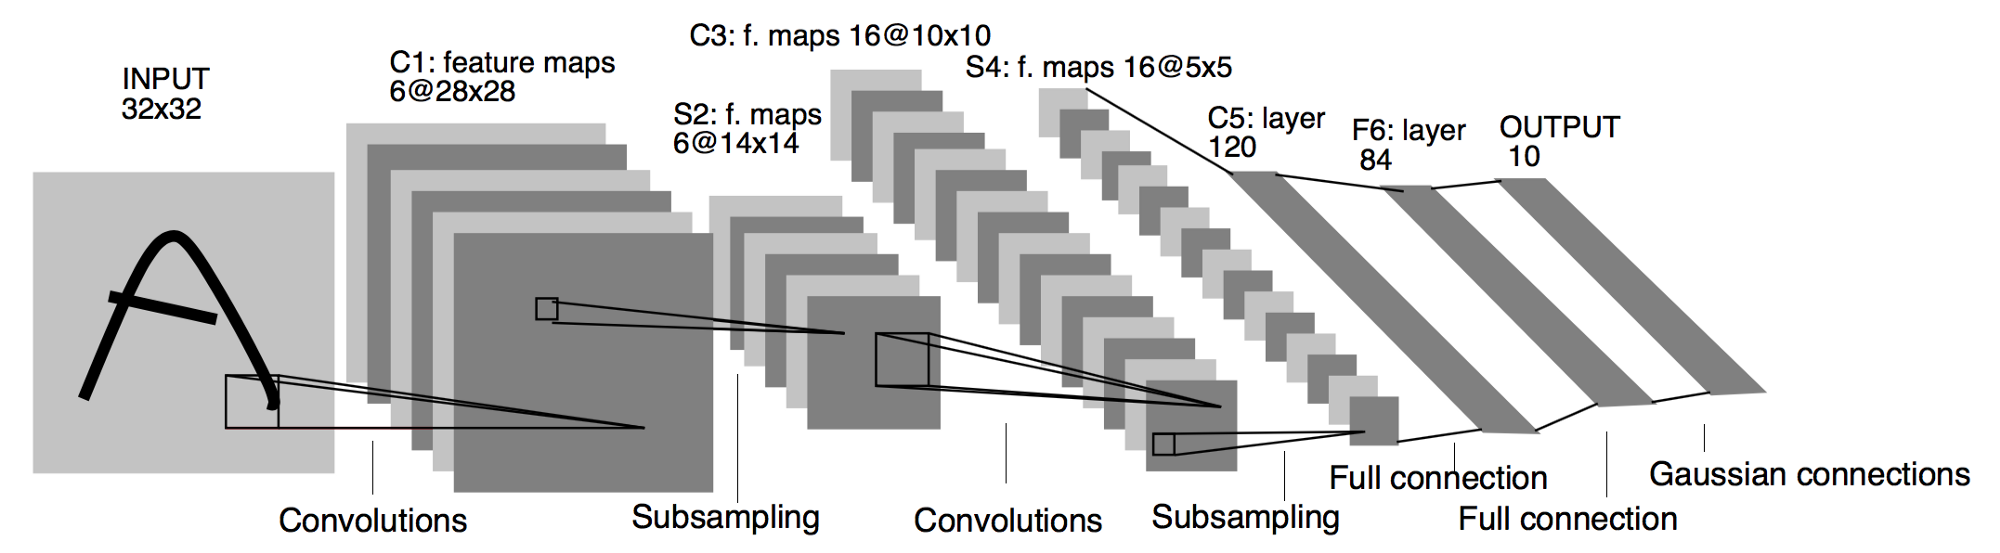
\includegraphics[width=0.8\textwidth]{images/ann_conv/lenet5.png}
	\caption{Als Beispiel für ein Convolutional Neural Network wird die LeNet-5 Architektur abgebildet. Entnommen aus \cite{lecunGradientBasedLearningApplied1998}  }
	\label{fig:lenet5}
\end{figure}
\vspace{0.2cm}
Angefangen mit der LeNet-5 \cite{lecunGradientBasedLearningApplied1998} Architektur, setzt sich typischerweise ein Convolutional Neural Network aus einer Sequenz von unterschiedlichen Layer-Arten zusammen \cite{szegedyGoingDeeperConvolutions2015, CS231nConvolutionalNeurala}. Im weiteren Verlauf dieses Kapitels werden die Arten der Layer beschrieben. Die Abbildung \ref{fig:lenet5} illustiert die LeNet-5 Architetkur als Beispiel für ein CNN. Die Tabelle \ref{tab:layer_param} gibt eine Übersicht der Layer und ihrer Parameter an.

\vspace{0.1cm}
\begin{table}[H]
	\centering
	\caption{Übersicht der Parameter und Hyperparameter der Layer eines Convolutional Neural Networks. Die Parameter werden während der Trainingsphase optimiert und Hyperparameter werden zuvor fest definiert \cite{yamashitaConvolutionalNeuralNetworks2018}. }
	\begin{tabularx}{1.0\textwidth}{X X X}
		\textbf{Art des Layers} & \textbf{Parameter} & \textbf{Hyperparameter}\\
		\hline
		Convolutional Layer & Filter & \makecell[tl]{
			Filtergröße\\
			Anzahl der Filter (\textit{Tiefe})\\
			Stride\\
			Padding\\
			Aktivierungsfunktion
		}\\
		\hline
		Pooling Layer &  \textit{keine}  & \makecell[tl]{
			Pooling Methode\\
			Filtergröße\\
			Stride\\
			Padding
		}\\
		\hline
		Fully-Connected Layer & Gewichte & \makecell[tl]{
			Anzahl der Gewichte\\
			Aktivierungsfunktion
		}\\
		\hline
	\end{tabularx}
	\label{tab:layer_param}
\end{table}
\pagebreak
\subsubsection{Convolutional Layer}
Der Convolutional Layer ist der Hauptbestandteil eines CNNs, der die Kombination einer Convolution Operation und einer Aktivierungsfunktion ist \cite{yamashitaConvolutionalNeuralNetworks2018}.

Die Convolution Operation basiert auf die mathematische Faltung (\textit{Convolution}) und wird typischerweise in CNNs, mit Verzicht auf die Kommutativität, der anliegenden diskreten Kreuzkorrelation gleichgesetzt \cite{Goodfellow-et-al-2016}.

Sei $I$ ein 2D-Input, $K$ ein 2D-Filter der Größe $M \times N$, $S$ die Schrittweite (\textit{Stride}) und $O$ das Output mit der Größe $X \times Y$, dann ist die Convolution Operation mathematisch definiert als \cite{Goodfellow-et-al-2016}:
\begin{equation}
	\label{eq:convolution}
	O(x,y) = (I * K)(x,y) = \sum_{m}\sum_{n}I(S_x \cdot x+m, S_y \cdot y+n)K(m,n)
\end{equation}
Abbildung \ref{fig:convolution_layer} illustriert eine beispielhafte Convolution Operation.

Die Randbehandlung des Inputvolumens wird \textit{Padding} genannt. Es gibt eine Reihe von Padding Methoden. CNNs setzen grundsätzlich das Zero-Padding Verfahren ein. Das Zero-Padding Verfahren erweitert den Rand  des Inputvolumens um eine beliebige Breite und Höhe mit Nullen \cite{CS231nConvolutionalNeurala}. 

Die Werte des 2D-Filters stellen die \textit{Gewichte} dar und werden in der Trainingsphase optimiert. Ein Convolutional Layer kann aus mehreren 2D-Filter der gleichen Größe bestehen. Die Convolution Operation wird je 2D-Filter unabhängig auf die Schichten des Inputvolumens ausgeführt \cite{CS231nConvolutionalNeurala}. Das Output des Convolution Operation wird auch \textit{Feature Map} genannt. Die Tiefe des Feature Maps ist gegeben durch die Anzahl der 2D-Filter \cite{yamashitaConvolutionalNeuralNetworks2018}.

Prinzipiell wird das Output des Convolutional Layers durch die Übergabe des Feature Maps an eine Aktivierungsfunktion bestimmt.  Abbildung \ref{fig:relu} stellt eine Aktivierungsfunktion dar.

\begin{figure}[H]
	\centering
	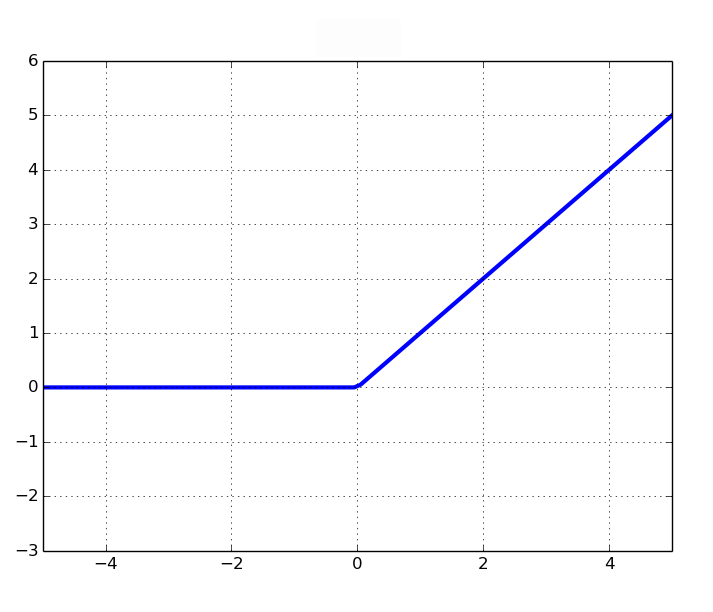
\includegraphics[width=0.4\textwidth]{images/ann_conv/ReLU.png}
	\caption{Ein Beispiel für eine Aktivierungsfunktion. Die ReLU (\textit{rectified liniear unit}) Aktivierungsfunktion wird typischerweise in CNNs eingesetzt und ist mathematisch definiert als: $f(x) = max(0,x)$ \cite{Goodfellow-et-al-2016} }
	\label{fig:relu}
\end{figure}

\pagebreak
\vspace*{\fill}
\begin{figure}[H]
	\centering
	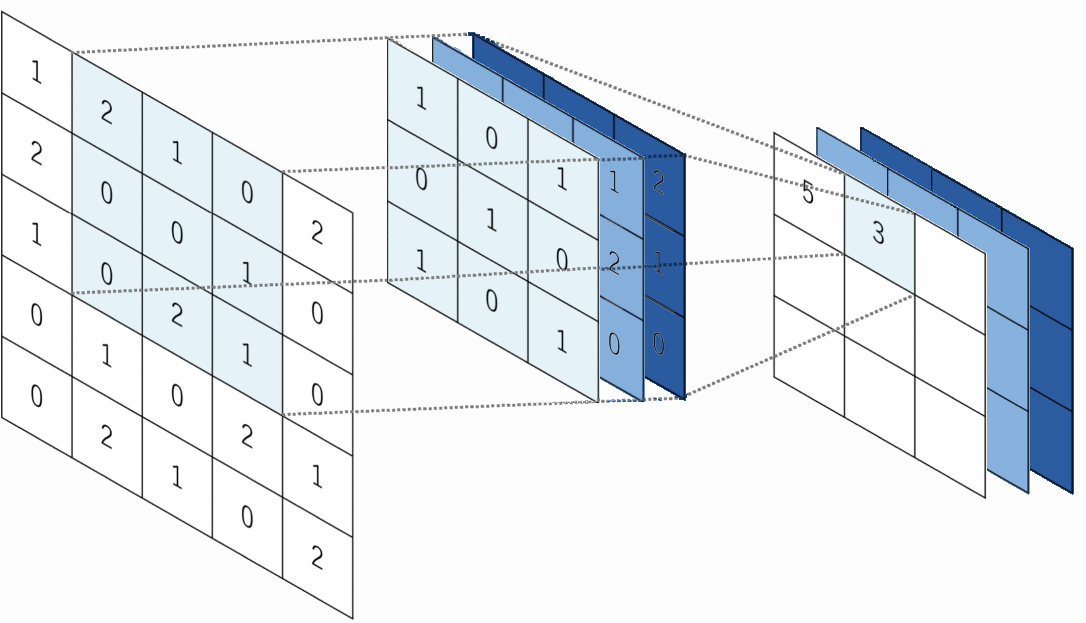
\includegraphics[width=0.8\textwidth]{images/ann_conv/convolution_layer.png}
	\caption{Ein Beispiel für die Convolution Operation mit 3 Filtern der Größe 3 $\times$ 3, je einem Stride von 1 und keinem Padding. Ein Filter bewegt sich entlang des gesamten Inputs mit der Schrittweite (\textit{Stride}) 1 und bildet die Summe der elementweise multiplizierten Werte. Die Summe wird dann im Feature Map an die korrespondierende Position geschrieben. Dieser Vorgang wiederholt sich für jedes Filter \cite{yamashitaConvolutionalNeuralNetworks2018}. }
	\label{fig:convolution_layer}
\end{figure}
\vspace*{\fill}
\pagebreak
\subsubsection{Pooling Layer}
Auf einen Convolutional Layer folgt i.d.R. ein Pooling Layer. Pooling Layer reduzieren die Größe eines Inputvolumens und verringern somit die Anzahl der erlernbaren Parameter \cite{CS231nConvolutionalNeurala}. Daher werden sie in der Literatur oft auch als \textit{Supsampling} Layer bezeichnet. Die Pooling Operation wird auf jeder Schicht der Eingabe ausgeführt \cite{CS231nConvolutionalNeurala}. Die meist verbreitete \textit{Pooling Methode} ist die Max-Pooling. Beim Max-Pooling iteriert ein Filter einer bestimmten Größe mit einer Schrittweite, gegeben durch den Stride, über das Inputvolumen und extrahiert das Maximum im aktuellen Filterbereich. Das Maximum wird für die weitere Berechnung beibehalten und die restlichen Werte verworfen
 \cite{CS231nConvolutionalNeurala}. In dieser Arbeit wird neben der Max-Pooling Operation auch die Average-Pooling Operation eingesetzt. Das Average-Pooling behält im aktuellen Filterbereich den Durchschnittswert, statt das Maximum \cite{CS231nConvolutionalNeurala}.
 
 Im Vergleich zu einem Convolutional Layer wird ein Pooling Layer nur aus Hyperparameter definiert und bleibt daher statisch \cite{yamashitaConvolutionalNeuralNetworks2018}. Abbildung \ref{fig:pooling_layer} zeigt eine beispielhafte Ausführung einer Max-Pooling Operation. Tabelle \ref{tab:layer_param} listet die Hyperparameter eines Pooling Layers auf.
 \vspace*{1cm}
 \begin{figure}[H]
	\centering
	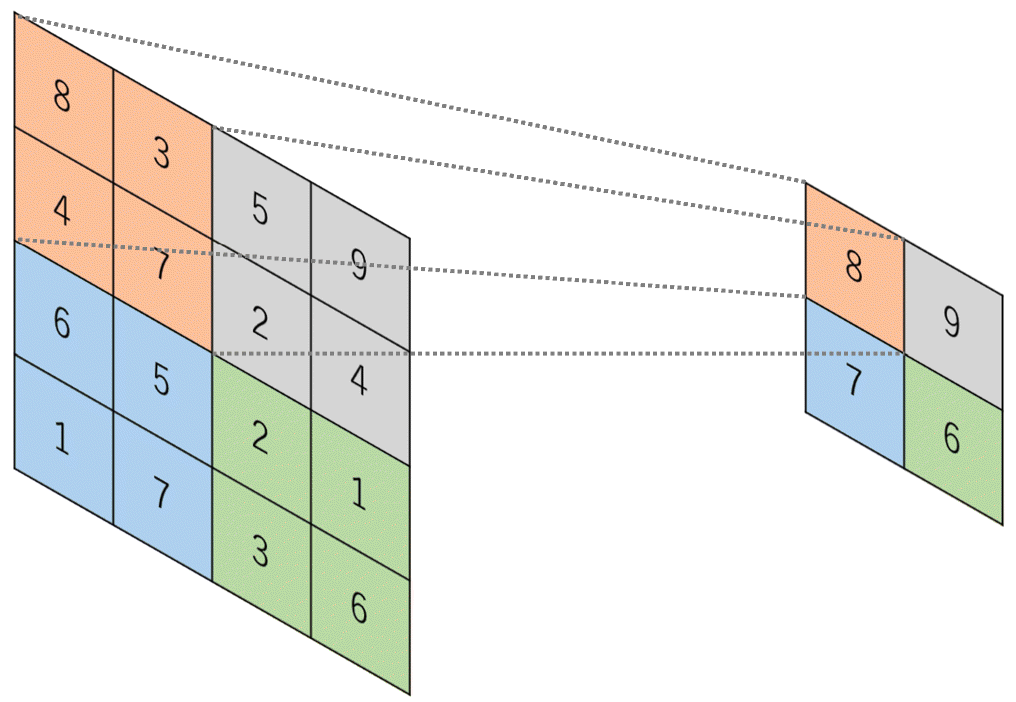
\includegraphics[width=0.6\textwidth]{images/ann_conv/max_pool.png}
	\caption{Ein Beispiel für eine Max-Pooling Operation mit einer Filtergröße von 2 $\times$ 2, einem Stride von 2 und keinem Padding. In diesem Beispiel wird der Input in 2 $\times$ 2 Bereiche unterteilt und der Maximum jedes Bereiches als Output berechnet. Es werden die markantesten Werte einer Nachbarschaft behalten und der Rest verworfen. Diese Operation führt zu einer Reduzierung der Inputgröße um den Faktor 2. Entnommen aus \cite{yamashitaConvolutionalNeuralNetworks2018}.}
	\label{fig:pooling_layer}
\end{figure}



\subsubsection{Fully-Connected Layer}
Nach einer Periode von Convolution- und Pooling Layer folgt meist ein fully-connected (\textit{FC}) Layer, auch bekannt als \textit{Dense Layer}. Dieser Layer folgt dem gleichen Konzept der feedforward Neural Networks, wie in Abschnitt \ref{sec:feedforwardNN} beschrieben. Das Output dieses Layers wird häufig einer weiteren Aktivierungsfunktion übergeben \cite{yamashitaConvolutionalNeuralNetworks2018} und prinzipiell wird dadurch das Output des CNNs bestimmt.

\subsection{Bekannte CNN Modelle}
Es existiert eine Menge von bekannten CNN Modellen mit ausgezeichneten Ergebnissen in internationalen Wettbewerben, derartige wie z.B. die ImageNet Large Scale Visual Recognition Challenge (\textit{ILSVRC}) \cite{russakovskyImageNetLargeScale2015}. Dieser Arbeit behandelt nur die Architektur des GoogLeNet Modells und dessen Modifikation PoseNet.

\subsubsection{GoogLeNet}
\label{sec:googlenet}
GoogLeNet, konstruiert von \citet{szegedyGoingDeeperConvolutions2015} im Jahr 2014, ist der Sieger des ImageNet Large Scale Visual Recognition Challenge (\textit{ILSVRC}) 2014 Wettbewerbes. Die ILSVRC stellt ungefähr 1000 Bilder aus 1000 unterschiedlichen Kategorien aus der ImageNet Datensatz bereit. ImageNet ist eine Bildersammlung bestehend aus über 14 Millionen manuell annotierten Bildern in über 20 Tausend unterschiedlichen Kategorien. Die Herausforderung von ILSVRC ist, die 1000 Objekte bestmöglich auf den Bildern zu klassifizieren.

GoogLeNet ist eine besondere Inkarnation des sogenannten\textit{ Inception Moduls}, das zeitgleich mit GoogLeNet vorgestellt wird.
Ein Inception Modul beinhaltet mehrere Convolutional- sowie einen Pooling Layer und verarbeitet das Inputvolumen parallel auf 4 Zweigen. Vor rechenintensiven Convolutional Layer werden zusätzliche 1$\times$1 dimensionsreduzierende Layer geschaltet. Abschließend werden die Zweige, die ein Volumen mit der gleichen Breite und Höhe produzieren, zu einem Outputvolumen (in die Tiefe) zusammengeführt.  Durch die parallele Berechnung der Zweige und das Einschalten von dimensionsreduzierenden 1$\times$1 Layer vor rechenintensiven Operationen ermöglicht ein Inception Modul neuronale Netze, bei zunehmender Tiefe und Breite, konstante Rechenkapazität zu verlangen \cite{szegedyGoingDeeperConvolutions2015}.
Inzwischen wurde das Inception Modul \cite{szegedyRethinkingInceptionArchitecture2016} und die gesamte Architektur rundherum \cite{szegedyInceptionv4InceptionResNetImpact2016} weiterentwickelt. Abbildung \ref{fig:inception_module} stellt das Inception (\textit{v1}) Modul dar.

Die Architektur von GoogLeNet besteht aus 9 Inception Modulen (je von Tiefe 2) und hat eine gesamte Tiefe von 22 Layer \footnote{Anzahl der trainierbaren Layer inkl. Output Layer}. Das Ungewöhnliche an der Architektur ist, dass es 3 Output-Zweigen hat. Jedes der Ouput-Zweige produziert ein Klassifizierungsergebnis. Output-Zweig 2 \& 3 sind Hilfszweige, die nur in der Trainingsphase einen Einfluss haben und in der Evaluationsphase verworfen werden \cite{szegedyGoingDeeperConvolutions2015}. Abbildung \ref{fig:googlenet} illustriert die GoogLeNet Architektur in Detail.

\vspace*{\fill}
 \begin{figure}[H]
	\centering
	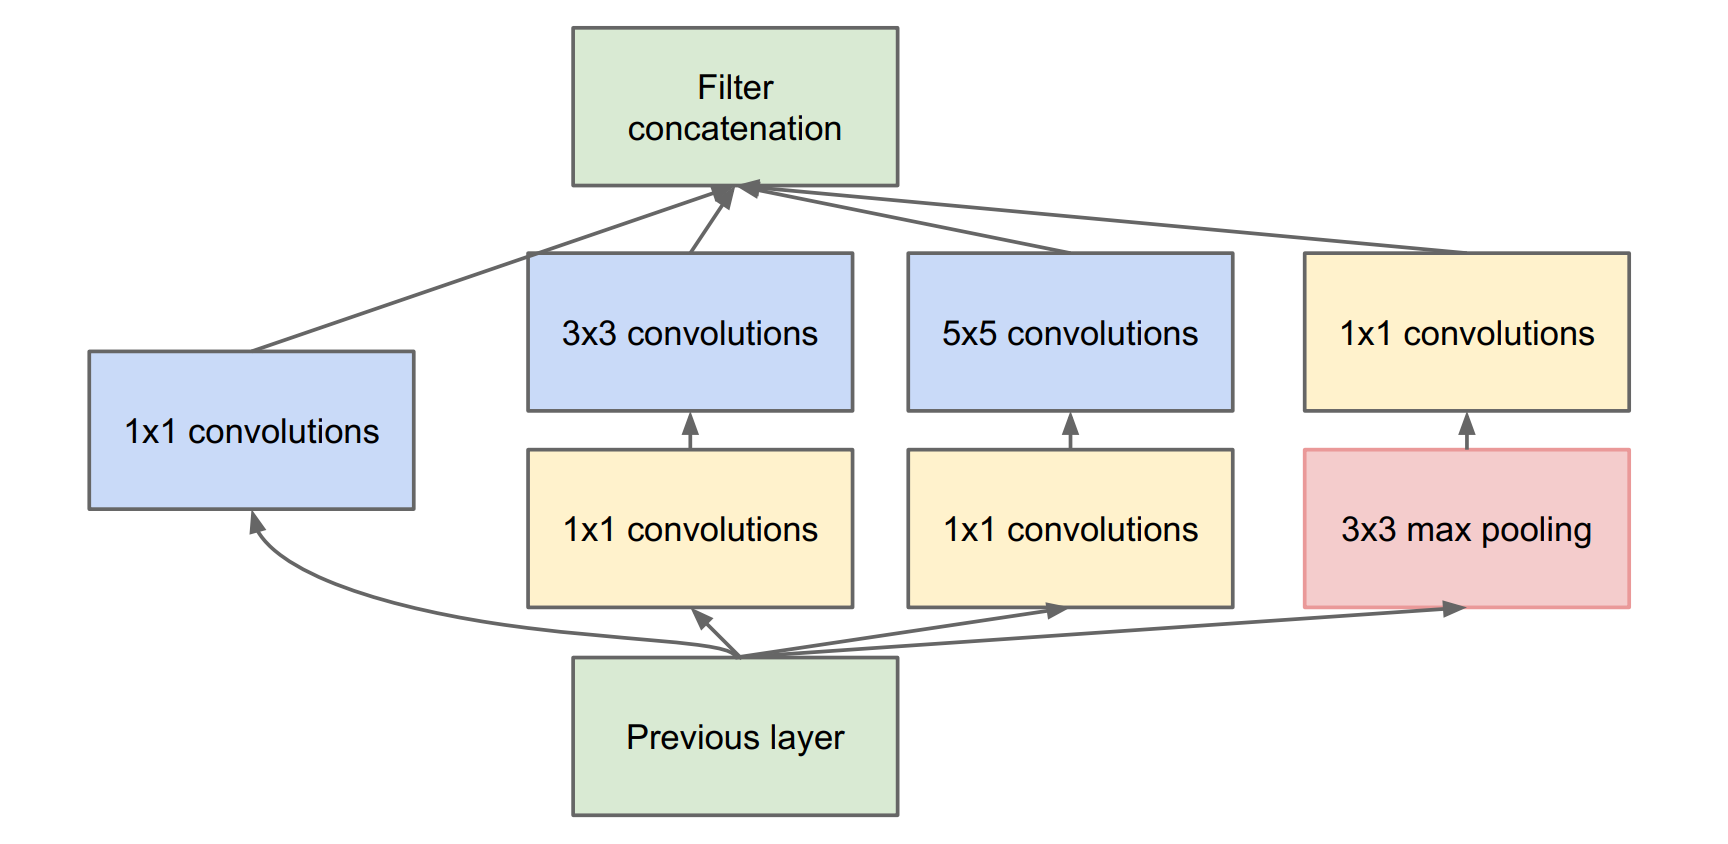
\includegraphics[width=0.8\textwidth]{images/googlenet/inception_module.png}
	\caption{Darstellung des Inception (\textit{v1}) Moduls. Das Inputvolumen wird auf 4 Zweige unabhängig verarbeitet. Die Ergebnisse der unabhängigen Operationen haben die gleiche Breite und Höhe. Das Output des Inception Moduls wird durch das Konkatenieren (in der Tiefe) der einzelnen Ergebnisse bestimmt. Die gelben 1$\times$1 Convolutional Layer dienen zur Dimensionsreduktion. Entnommen aus \cite{szegedyGoingDeeperConvolutions2015}.}
	\label{fig:inception_module}
\end{figure}
\vspace*{\fill}
\pagebreak

\vspace*{\fill}
	 \begin{figure}[H]
		\centering
		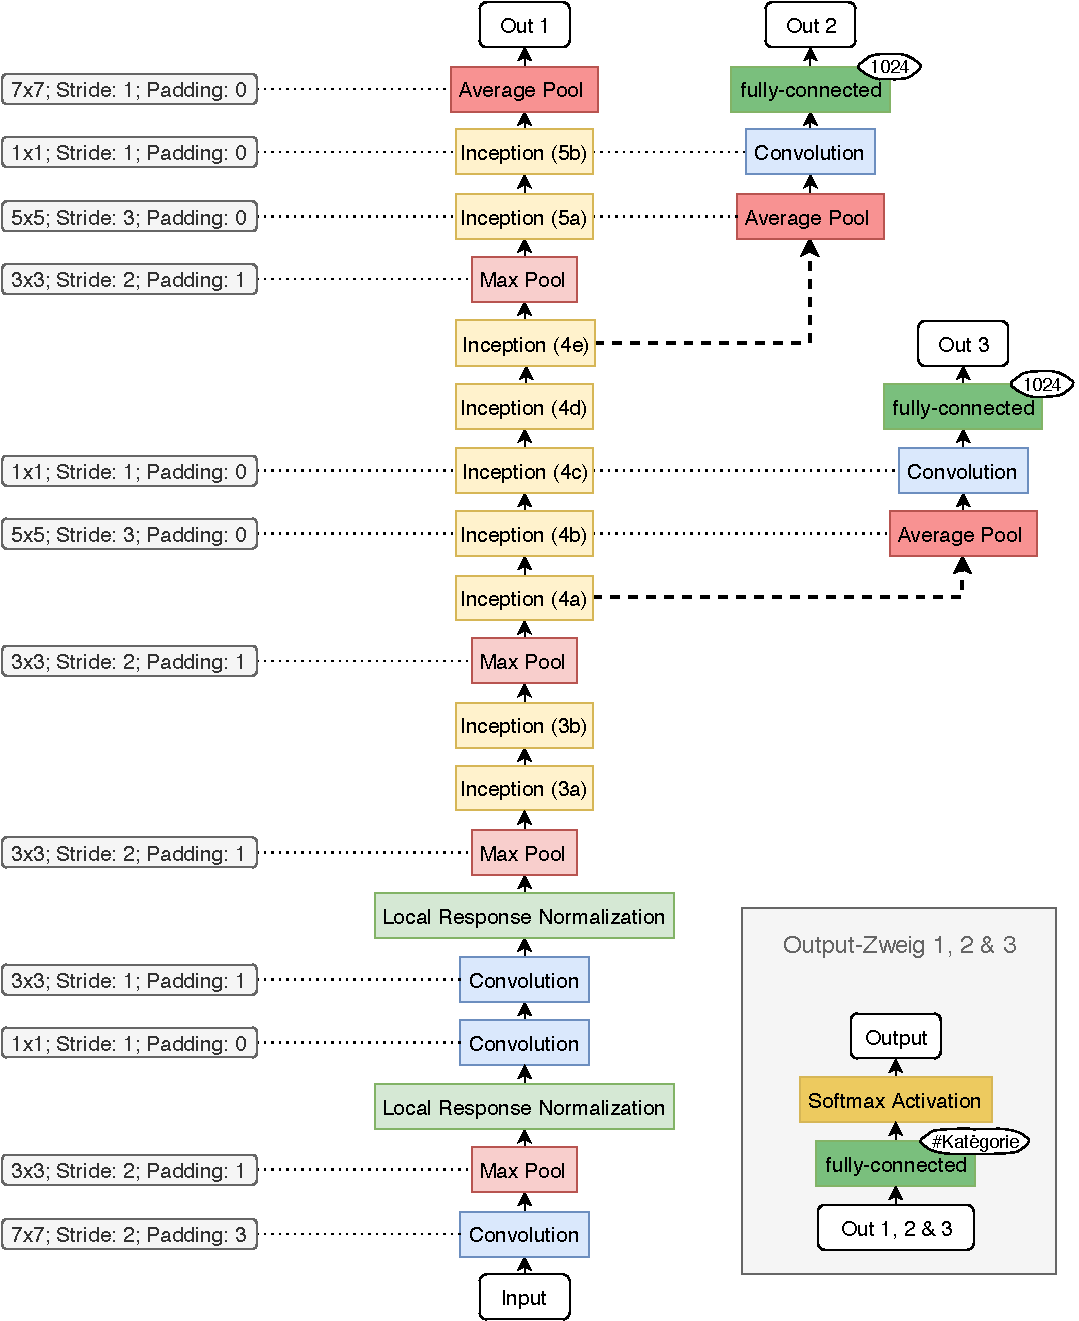
\includegraphics[width=0.85\textwidth]{images/googlenet/googlenet_diagram.pdf}
		\caption{Der architektonische Aufbau des GoogLeNet Models. Das Inception-Block wird in Abbildung \ref{fig:inception_module} detaillierter dargestellt. Es gibt 3 Ouput-Zweige, die mit einer identisch aufgebauten Output-Knoten enden. Die Werte der Output-Zweige 2 \& 3 haben nur während der Trainingsphase einen Einfluss und werden in der Evaluationsphase verworfen. In der Trainingsphase wird vor dem Output-Knoten 1 ein Dropout von 40\% und vor den Output-Knoten 2 \& 3 ein Dropout von 70\% angewandt. Jedes Convolutional Layer hat die ReLU (Abbildung \ref{fig:relu}) als Aktivierungsfunktion. Die \textit{Local-Response-Normalization} \cite{krizhevskyImageNetClassificationDeep2012a} ist ein bekanntes Normierungsverfahren und kommt prinzipiell in Verbindung mit der ReLU Aktivierungsfunktion vor. Abbildung basiert auf \cite{szegedyGoingDeeperConvolutions2015}.}
		\label{fig:googlenet}
	\end{figure}
%\vspace*{\fill}
%\pagebreak
\subsubsection{PoseNet}
\label{sec:posenet}
PoseNet, vorgestellt von \citet{kendallPoseNetConvolutionalNetwork2015} im Jahr 2015, basiert auf die im Kapitel \ref{sec:googlenet} eingeführte GoogLeNet Architektur. Statt eine Wahrscheinlichkeitsverteilung der Klassifizierungsergebnisse, liefert PoseNet die 6 Freiheitsgrade einer Pose $y = [\pmb{p};\pmb{q}]$, bestehend aus einem Positionsvektor $\pmb{p} \in  \mathbb{R}^{3}$ und eine Quaternion der Orientierung $ \pmb{q} \in  \mathbb{R}^{4}$.

PoseNet modifiziert die GoogLeNet Architektur an den Output-Knoten, dargestellt in Abbildung \ref{fig:googlenet}, wie folgt \cite{kendallPoseNetConvolutionalNetwork2015}:
\begin{itemize}
	\item Jedes der Softmax-Klassifikatoren werden ersetzt durch Regressoren. Dabei wird der Softmax-Activation Layer entfernt und der FC-Layer so modifiziert, dass es einen 7-dimensionalen Vektor\footnote{(3) für die Position und (4) für die Orientierung} ausgibt.
	\item Vor dem finalen Regressor des Output-Zweiges 1 wird ein weiteres FC-Layer der Breite 2048 eingefügt.

\end{itemize}
Abbildung \ref{fig:posenet_mods} veranschaulicht die Modifikation von GoogLeNet durch PoseNet.
\vspace*{1.2cm}
 \begin{figure}[H]
	\centering
	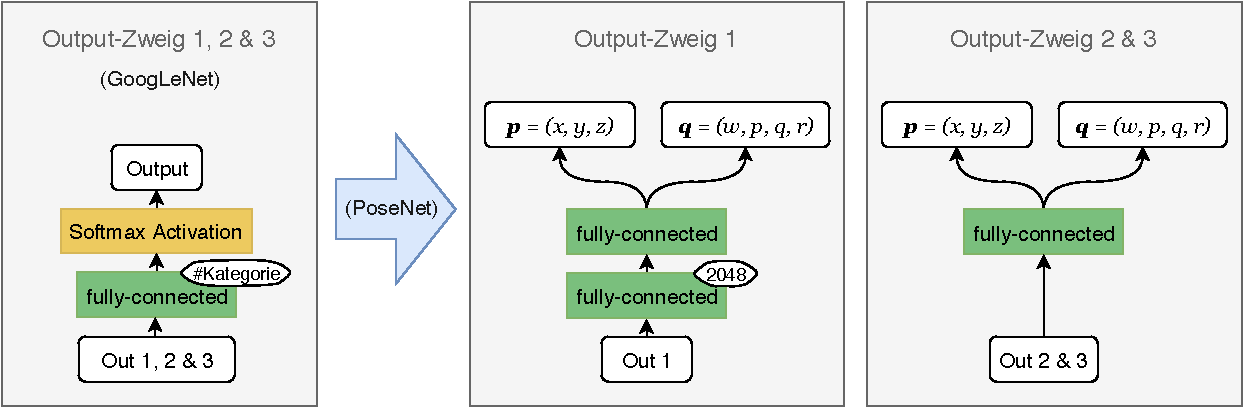
\includegraphics[width=\textwidth]{images/googlenet/posenet_diagram2.pdf}
	\caption{Veranschaulichung der Modifikation von den Output-Zweigen der GoogLeNet Architektur durch PoseNet. Die Softmax Aktivierungsfunktion sowie das fully-connected Layer mit Anzahl der Klassifizierungskategorien als Breite wurde von allen Output-Modulen entfernt. Jeder Output-Zweig hat einen FC-Regressionsschicht erhalten, dass die 6 Freiheitsgrade einer Pose bestimmt. Der Output-Zweig 1 wird zusätzlich mit einer weiteren FC-Layer der Breite 2048 vor dem Regressionsschicht erweitert \cite{kendallPoseNetConvolutionalNetwork2015}.}
	\label{fig:posenet_mods}
\end{figure}
\vspace*{1.5cm}

Die Autoren \citet{kendallPoseNetConvolutionalNetwork2015} stellen zusätzlich eine neue Kostenfunktion, mit den Parametern $\hat{y} = [\hat{\pmb{p}};\hat{\pmb{q}}]$ als Soll-Wert und $y = [\pmb{p};\pmb{q}]$ als Ist-Wert, vor:
\begin{equation}
	\label{eq:posenet_loss}
	loss(I) = \norm{ \hat{\pmb{p}} - \pmb{p} }_2 + \beta \norm{ \hat{\pmb{p}} - \frac{\pmb{q}}{\norm{\pmb{q}}}}_2
\end{equation}
Der Hyperparameter $\beta$ soll eine Balance der Kosten zwischen dem Positions- und Orientierungsdiskrepanz darstellen und wird in Gebäuden im Wertebereich zwischen 120 bis 750, sowie außerhalb des Gebäudes zwischen 250 bis 2000, empfohlen \cite{kendallPoseNetConvolutionalNetwork2015}. 